\chapter{Discussion}
\label{chap:discussion}

In this chapter we will provide a discussion of the findings done in the two workshops we have conducted, and on the concept we have created. The findings and results will be discussed up against theory and previous studies, as well as with our own opinions. 

In Section \ref{sec:discfindings1} we will discuss the findings from workshop 1 together with the theory discussed in previous chapters. This will be related to our choice of system requirements and exergame concept. In this way, the reasons for the choices made should become evident to the reader. In Section \ref{sec:discfindings2} we will discuss the findings from workshop 2, and based on this, provide a list of recommended improvements and adjustments for the game. During our study, we became aware that there was a problem with delay in some of the commercial games. This was an issue that was discussed and commented on several times by the informants. Therefore, we will, in Section \ref{sec:delay}, provide a brief discussion of this issue, and direct the interested researcher to relevant references on this topic. At last in this chapter, we will discuss the quality of the research. This can be found in Section \ref{sec:qualityofresearch}. 

\section{Discussion of Gathered Data and its Relation to the Exergame Concept}
\label{sec:discfindings1}

In Section \ref{sec:usability} we discussed the importance of usability which is about how easy a system is to use, learn and understand. Workshop 1 was performed to see how a set of relevant users interacted with commercial exergames, and to identify which aspects of these games that do or do not work for this user group. Three relevant elements that are used to measure a system's usability are: \emph{effectiveness}, \emph{efficiency}  and \emph{satisfaction}. These were aspects among others which we tried to measure in this workshop. We also tried to answer the exergame's \emph{context of use}. We were seeking to discover the needs of the intended users, the need for functionality, and the environment for the game. Where and in which circumstances the game can be used were discussed in our previous project assignment \cite{project}. This is not the main focus in this thesis, but it will briefly be discussed, as it was commented by the informants.

In this section, we will discuss findings from workshop 1, and relate these findings to the literature provided in previous chapters. From this we will emphasise what we have considered in our exergame concept. With the findings from workshop 1 and the literature study conducted we want to answer these two research questions: 

\emph{RQ1: Are existing commercial Xbox Kinect games suitable for exercising purpose for elderly people?}

\emph{RQ2: What are the design challenges when developing an exergame for elderly people, and what aspects need to be considered in this game?}

We will start with a general discussion, before we at the end of this section provide a summary to more precisely answer these two research questions. 

\subsection{Control of Character, Clear Goals and Feeling of Mastery}
The GameFlow model \cite{sweetser}, discussed in Section \ref{sec:heur}, describes eight core elements that should be present to experience enjoyment in games. One of these elements is control. The informants expressed that they did not feel they had control over their character. This was due to the significant delay that was present in the games. In addition, it came clear from the observation that it was not always easy to understand when the game started and ended, as well as what was an instruction video and what was the actual game. Clear goals did also seem to lack in the commercial games, and it was expressed by one informant that there was a need for more instructions on the rules of the game, and on what was expected from them. In Section \ref{sec:sergames}, we discussed how video games can function as a pedagogical tool and it was shown that important factors to focus on include motivation, effectiveness and intuitiveness. These aspects were also mentioned by the informants. They expressed that the system needs to be easy to understand, and that it is important to see a learning curve, and experience a feeling of mastery. In Section \ref{sec:motivators}, self-efficacy is described as an important determinant for exercise behaviour. Elements that are relevant to sustain this exercise behaviour are the feeling of pleasure and satisfaction, and self-regulatory skills. This was also discussed in workshop 1 as important aspects, and the informants mentioned goal setting, the possibility for socialising, and the possibility to decide for themselves what to do, as important. The feeling of mastery was seen as significant, and the informants were clear that if they did not get the feeling of mastery, they would not play these games. This relates to the elements discussed in the GameFlow model \cite{sweetser}, which states that games should include challenges matching the player's skills, different levels of challenges, and clear goals, to ensure player enjoyment. 

In our exergame we have emphasised the inclusion of different difficulty levels. This has been done in two ways: Different initial difficulty levels the player can choose between, and different difficulty levels within the initial levels, where the next level depends on the previous. In addition, clear goals, with appropriate challenges where the player will be rewarded with points, are aspects that are highly considered in the exergame.  

Clear instructions are included in our exergame to let the player know what is expected from her, and for her to know when the game starts and stops. In this way the player should feel she is in control of the game. We are not in control over the technical details, like delay and response time. However, this should be improved for the player to feel control over their character.
 
\subsection{Immersion and Concentration}
As presented in the GameFlow model \cite{sweetser}, immersion and concentration are important aspects of the gaming experience. It was hard to evaluate from observing and interviewing the informants if they were immersed into the game and concentrated on the tasks. However, comments from the informants during game play, like \emph{"I felt like the avatar itself"}, and \emph{"I wanted that pineapple"}, suggest that the informants immersed into the game. If we are to evaluate, we would say that all the games required concentration to perform the tasks right. However, it did not always seem like the informants were that concentrated. A few times, we had to assist the informants in reading messages appearing on the screen, like "raise hand above head to play", while they at other times read the same type of messages by themselves. We believe that the text should have been clear enough, and that the reason for them not reading the text, was because they did not concentrate enough on the game. 

Concentration and immersion are considered in our exergame. For the player to see obstacles on the trail, as well as to see when apples ripen, they need to concentrate. We have provided an intuitive interface with simplistic design, which makes it easy to concentrate on important elements and tasks. The activities in the exergame are provided in a real-life environment well known for elderly, and are based upon activities suggested as interesting for them. In addition, the exergame is presented with 3-dimensional graphics. This has been done to enhance the players immersion into the game, and hence increase the gaming experience.

\subsection{The Possibility to Customise}
We have learned from guidelines presented in Section \ref{sec:summaryguidelines}, and from the informants, that there is a need to customise an exergame aimed for elderly users. This is to be able to meet various limitations and disabilities they might have. Our previous project \cite{project} supports this need for customisation. There we evaluated the game to fit as a tool for physiotherapists to use as an alternative exercise method. What this game should offer was therefore described as: \emph{"A tool with the ability to customize an exercise program, and to offer an alternative, fun and motivating training method, while at the same time ease the workload of the physiotherapist"} \cite{project}. The possibility to customise the exergame can be a feature in the physiotherapists' interface, where they can put together different exercises within the game story, which fits their patient's needs. They could also set parameters to adjust difficulty levels according to progress, set the pace in the game to ensure mastery, and also change font and background to preferred size and colour to ensure readability. Another example is for the user herself to have an interface where she can put together her own program and set her own parameters. We have made requirements for this; however we have limited our thesis to not design an interface with the possibility to customise. These requirements are represented as 1.33, 1.34, and 1.35 in Table \ref{tab:func3}. Requirements 1.31 and 1.32 say that the system should have user profiles where players' progression and results can be saved. This profile should be possible to share with others. This will be especially important in a clinical setting, for the physiotherapist to monitor the patients' progress. We have not included this user profile in our concept either. The development of a user-interface seen from the physiotherapists, as well as the user profile, will be left for future work. 

As discussed in our previous project, the game should, in the future, be used for home based training \cite{project}, handed out by the physiotherapist. This can overcome some challenges when it comes to motivating elderly to exercise. First, as discussed in Section \ref{sec:barriers}, one challenge about getting elderly to exercise, is if the person lives far away from training facilities. This was also mentioned by one informant. Second, another informant mentioned that she did not want to be controlled by time and appointments. An exergame implemented at home would make exercising convenient and more available. If physiotherapists use this game as a home training program, different prompts, as suggested in Section \ref{sec:motivators}, should be used as follow-up. 

\subsection{Social Aspects}
The GameFlow model says that games should support social interaction to meet player enjoyment. Also in Section \ref{sec:exergames} the importance of social interaction in exergames are discussed, and in \cite{statistics2012} it is stated that as much as 62 percent of all gamers say they play with others, either together in the same room or online. Guidelines presented in Section \ref{sec:summaryguidelines} also suggest inclusion of social factors in a game for elderly. Offering social interaction, is especially important for elderly who experience loneliness in their everyday life, due to inactivity \cite{exergamesforelderly}. It was interesting to learn that social interaction also was seen as important by the informants. The majority of the informants would rather play together than alone. They mentioned playing together in a group setting, and especially, playing together with grandchildren. However, none of the informants could see themselves playing together with others over the Internet. This relates to findings done in \cite{Gajadhar}, where it was shown that elderly enjoyed playing together in the same room more than playing online. We believe that one of the reasons why the informants stated this was because they did not understand the concept of "playing over the Internet", as a result of their inexperience with this technology. This assumption is supported by one of the characteristics in Section \ref{subsec:characteristics}. This might indicate that the market is too immature for this. However, having this way of gaming introduced by grandchildren may remove some barriers related to playing over the Internet. Especially, if they get to understand that online gaming could mean more contact with their family. Presenting a picture of the co-player in a corner of the screen might help the elderly draw relations and increase the feeling of socialisation. We did not include this in our exergame. However, this should be looked into in future work.


Two informants meant it was more motivating to collaborate than to compete. This was also found in \cite{Gajadhar}, where they, based on results from their study and from studies conducted by others, conclude that the focus should be on collaborative play rather than competition for this group of people. However, the other informants seemed to like both to collaborate and to compete. In our exergame, we have provided both the possibility to compete and collaborate, because of two reasons: First, several of the informants wanted the possibility to play together with grandchildren. The findings done in \cite{Gajadhar} shows that elderly prefer to collaborate and help each other, rather than to compete. This is in contrast to what they found in previous studies about young people, which is that young people prefer competition. And second, the majority of the informants seemed to want the possibility to choose. 

\subsection{Appropriate and Simple Feedback and Information}
The informants included in our research were relatively physically and mentally fit. However, we found some informants to meet some of the typical characteristics of elderly, listed in Section \ref{sec:summaryguidelines}. We experienced that one of the informants had problems reading the text in some of the menus. Because it was only one informant that had problems with this, we assume that this informant might have had impaired vision. However, as discussed in Sections \ref{sec:summaryguidelines} and  \ref{sec:designelderly}, impaired vision is a common problem for the older population, and should be considered in a game designed for this group. This has been taken into account in our menu proposal. The group of informants had interest in technology and used a wide range of devices. However, none of the informants had any experience with video games. In the beginning of the workshop we experienced that the informants were insecure, and had problems understanding what they were supposed to do. It took some time for most of them to understand that they had to use their body to play. Therefore, we see the need for clearer instructions both before and during game play. This includes an introduction to how the system works, how to interact with the sensor, and information about what is expected from the player in the game. Clearer instructions have been defined as a requirement for our exergame. The final characteristic that we experienced was that some of the informants expressed that it was hard to do more than one thing at the same time. Therefore, the information given, and the tasks to be done, should be limited, and adjustable. The possibility to add more functionality after the existing functionalities are managed was suggested by one informant. This is also stated in the guidelines from Section \ref{sec:summaryguidelines}, and suits well with the requirements of simplicity discussed in Section \ref{sec:simplicity}. We have solved this by offering different difficulty levels. 

We learned from workshop 1 that the feedback presented in the commercial games did not satisfy the informants. Feedback is one important element from the GameFlow model, and are also stated as guidelines in Section \ref{subsec:golden} and \ref{sec:summaryguidelines}. These guidelines suggest that informative feedback should be given in a motivating form at appropriate times. The informants desired more feedback on their actions, and they especially wanted to know whether they did the exercises right or wrong. They did not feel that they got this feedback in the games played in the workshop, which made them both confused and frustrated. Some of the games had a lot of different features that were supposed to be motivating. However, this was perceived as rather annoying. In addition, the amount of the information given, both with text and voice, was experienced as too much. At the same time, some of the informants stated that they did not recognise these types of messages at all. In Section \ref{sec:simplicity}, we discussed minimalistic design which is about bringing the most important elements into focus, and avoiding elements that can distract the user. Microsoft presents it as "Simple Can Be Powerful", which means that simplistic design not necessarily needs to mean lack of functionality. From this we concluded that we should avoid too much features in our exergame. We have chosen to keep it simple, and to focus on a few motivating aspects, such as to see progress in the health-bar. One informant desired more time to read information and instructions, and suggested that there should be a way to tell the system when you are finished reading. This is supported by guidelines in Section \ref{sec:designelderly}, and has been taken into consideration in our exergame. The feedback is given at appropriate time when the player manages to do a task, and instructions on the task will be given as the task appears. In addition, the player can spend all the time she wants watching the instructions.

\subsection{Cultural and Lifestyle Diversity}
Guidelines from Section \ref{sec:summaryguidelines} and \ref{subsec:golden} are about the importance of matching cultural and lifestyle diversity in games. This was also expressed by the informants, and they suggested different type of themes for a possible game concept, like dance, swimming, apple picking etc. If they were to play a game like this they stated that it would need to include sports or activities related to real life. They also mentioned the importance of appropriate music. They did not like the music in the commercial games because it did not relate to the music they used to listen to. In Section \ref{sec:motivators} appropriate music is proposed to be a motivator for exercising, and in \cite{schutzer} it is discussed that music can be a way to divert from physical pain. This strengthens upon the importance of including music. The majority of the informants agreed that music was important, especially to keep the rhythm. However, they stated that they wanted it quiet, and they wanted music more related to their generation. This indicates that choosing the right music is an important requirement for the exergame. The informants' opinions did not differ much according to gender on what they liked and did not like in the games we tested. However, as discussed in Section \ref{sec:motivators}, different people's needs and expectations, as well as aspects such as gender and ethnicity should be considered. 

We have met cultural and lifestyle diversity by designing an exergame with a series of games that covers a variety of interests. In addition, the requirements specify that the player should be given the possibility to choose a male or female character. Race might also be considered, but it is difficult to cover all races. Chao et al. \cite{chao} discuss that to meet diversity requirements, it is important to be in contact with the relevant people. Even though we clearly have not covered the total group of elderly people, we have included a small group to understand some needs and expectations. Finding the appropriate music will be left for professionals, like music therapists. 

Observations made during workshop 1 identified some requirements that are not included in our exergame. This is related to the functionality and the hardware of the system. Elderly are, as mentioned, inexperienced with technology, and it is important for acceptance of an exergame, that the hardware is not too extensive and complicated. In addition, the load of introducing something new for this user group should be minimised. In this matter, they should be able to use the equipment they already have as much as possible. All of the informants had their own computers, and what would be most convenient would be to use these to play. This is possible, as the Kinect technology can be experienced with both the Xbox console and Windows computers, as we learned from Section \ref{sec:xbox}. This is discussed since it is important aspects of introducing an exergame for this user group. This, and additional non-functional requirements will be listed in Appendix J.  

\subsection{Summary}
We will now provide a summary of what we have discussed in this section, this to in a more precise way answer research questions 1 and 2. 

When reviewing related literature, presented in Section \ref{sec:relatedresearch}, it was discussed that existing commercial games are not aimed for the older user group. Based on this, different characteristics of elderly were discussed, and guidelines were suggested. That existing games are not suitable was also seen in our previous project \cite{project}, where studies found them to be too rapid and complicated for elderly. We wanted to explore this, by testing different commercial Xbox Kinect games to understand good and bad aspects within these games. Findings from this together with the previous research will answer research question 1:

\emph{RQ1: Are existing commercial Xbox Kinect games suitable for exercising purpose for elderly people?}

As mentioned initially, \emph{effectiveness}, \emph{efficiency}  and \emph{satisfaction} are relevant measurements when evaluating the usability of systems. Based on findings from workshop 1, we can conclude the following about the commercial games tested: 
\begin{itemize}
\renewcommand{\labelitemi}{$\bullet$}
\item The commercial games tested on a group of elderly do only to a degree meet the requirements of effectiveness. The functionality needed to play the game are present, however, the games do not spend enough time on instructions and information, and do not give sufficient feedback on whether the players' actions are done correctly. Because of the lack of instructions in "Fruit Ninja" it became clear that the informants did not understand what was required from them, and they just waved their hands uncontrollably. In addition, the delay problem weakens the functionality. The menus in "Aging with Grace" and "Fruit Ninja" do not need the requirement of effectiveness, as they are too complicated and there are too many elements present at the same time. The buttons are too sensitive, and it is not intuitive how to press them. The majority of the informants understood what was expected from them in the tennis game, and played through this game without problems. The skiing game was also well understood, until the second match where the two players that played together switched tracks. All of the informants had problems relating to their player after switching tracks. This also relates to the lack of instructions.
\item It is hard to evaluate the efficiency in a game, because it requires us to measure how much time used to accomplish a task. In these games, the players were forced to follow the pace in the game. All informants managed to complete the games, however, with various results. The efficiency of the two menus tested can be measured, as we can look at the overall time spend getting through them. The menus in "Aging with Grace" and "Fruit Ninja" do not meet the requirements of efficiency. We had to assist the informants through the menus, and because of too much information and too sensitive buttons, the informants spent unnecessary time on getting through the menus. In addition, the issue with the delay reduces the degree of efficiency.
\item Two of the four games played in workshop 1 meet the requirement of satisfaction. All of the informants liked playing the tennis and skiing game and they had fun while playing. "Fruit Ninja", they did not like that much, which relates to their wish for playing games with a meaningful content that they could relate to real life. The informants were not satisfied with "Aging with Grace" either, because this focused on "just" regular training, which they would rather do without the game. This supports Zyda's statement on that the main focus in serious games should be on fun and entertainment \cite{zyda2005visual}. 
\end{itemize}

It is important to remember that this was the first time the informants played games like these, and initially they did only play the games once \footnote{Three of the informants got to play the skiing game a second time because they specifically asked for it. We did not observe anything new in this second session, and have because of this, and because the rest of the informants did not try a second time, not included this in our analysis}, which do not enable us to say anything about the informants learning curve. However, we did see that they understood more what was expected from them, and that they got more confident after a while. If we had continued with several rounds with the same games, we might have seen improvements. This was also mentioned by the informants. 

To describe what is important to focus on when developing an exergame for elderly people, we will answer research question 2:

\emph{RQ2: What are the design challenges when developing an exergame for elderly people, and what aspects need to be considered in this game?}

Understanding the game's \emph{context of use} is important when specifying requirements. From the different characteristics discussed in Chapter \ref{chap:exforseniors}, and from meeting a group of relevant users, we have learned more about elderly as a group. The characteristics identified (see Section \ref{subsec:characteristics}) need to be acknowledged to make a suitable game. One of the main challenges when developing an exergame for this user group is that they are a group with diversity, both when it comes to interests and different types of disabilities. The informants desired a game with a story that appeals and relates to real life, as well as appropriate music to their age. Different themes for a possible game were mentioned, showing the diversity of needs. Guidelines proposed in Chapters \ref{chap:olderexercise} and \ref{chap:exforseniors}, as well as the Eight Golden Rules and the GameFlow model have many relevant elements that are found to be important. Several of the findings done in workshop 1 relate to these guidelines. From this we have made functional and interface requirements, which should be followed making an exergame for this user group. It was urged for more instructions on how to interact with the game, as well as what was expected from the players, the goals, and the rewards. The menus in the commercial games were seen as challenging because of the amount of information and the sensitive buttons. In a game for this user group this needs to be improved, taking physical disabilities in arms and visual decline into consideration. The majority of the informants would only play these types of games together with others. Social aspects are discussed as important in Section \ref{sec:summaryguidelines}, in the GameFlow model and by the informants. Therefore, this is included in our game. The delay in the games was seen as a great issue, and should be acknowledged. We believe that if this game is to be used for exercising, both at home and in clinical settings, technical precision has to be present. The last part of specifying the context of use, is to find out where and in which circumstances the users would like to use the game. In a previous study \cite{project} we evaluated the game to fit well as a part of physiotherapy or in a group training setting. This was supported by the informants. Most of them preferred playing with others, and could see this as an activity done together in a group. They also wanted to play the game with grandchildren.

It is important to acknowledge the difficulties about engaging a user group into a setting they are completely unfamiliar with. Most elderly are inexperienced with video game technology, and it could therefore be challenging to include them in a development process for an exergame. Not only is the technology completely new for them, but they have not yet acknowledged that this is something they are in the need for. We experienced some of these challenges in our workshop. The informants were involved with a new technology, and they were discussing an unfamiliar topic. This resulted in them at times being ambiguous in their feedback and comments. First, they said that they wanted to buy such a game, and few moments later they said that video games are a waste of time. We have tried to bring out the informants overall opinions during the workshop. 


\section{Evaluation of the Exergame}
\label{sec:discfindings2}
In Section \ref{sec:userinvolvement} we presented the importance of user involvement during system development, as the end-users are the ones who will use the final product, and are the only ones who know what they want. After creating an exergame based on specified requirements, we invited a group of elderly to a second workshop to get feedback on our ideas and design proposals. We presented prototypes of the exergame, and we opened up for questions and discussions. Figure \ref{userdesign} shows the cycle for user-centered design, where workshop 2 is about the fourth activity, which is to evaluate system design. As presented in Section \ref{sec:userinvolvement}, ISO 9241-210, states that feedback from users will help designers not only evaluate design, but also improve them according to the users' needs. Involving the end user in the design process will increase the possibility of making a user-friendly interface for the intended user group, which is, as stated in Section \ref{sec:usability}, crucial for making a successful system. 

In this section the evaluation of the exergame will be discussed. Based on theory and findings from workshop 2 we will present important aspects to be included in future work of designing this exergame for elderly. These aspects will be discussed, but we will not make any changes to our current exergame. This is out of the scope of this thesis and is left for future work. At the end, we will review what has been presented in this section, and use this to evaluate the exergame by answering research question 3:

\emph{RQ3: What would be suitable system requirements, and appropriate design, for an exergame for elderly people?}

\subsection{Few Comments and Moderate Response}
Generally there were few comments, but several questions, during the workshop. When we presented the various prototypes, the informants responded with silent nodding or just looking mutely at the screen. There could be several reasons for this. One reason could be because the informants were inexperienced with video game technology, which could have made it difficult for them to comment on the exergame, as they did not know what to look for and respond to. One informant stated that it was impossible for her to comment on the exergame, as she did not know anything about how the game would work. The moderate response could also be related to the informants' health conditions, and the fact that elderly see is at challenging to comprehend and process too much information at the same time. However, we found our informants to be both physically and mentally fit. 

Another reason for the lack of comments could be related to how we presented the prototypes. Our exergame is based on highly interactive video game technology, and it is, as presented in Section \ref{sec:prototypes}, very difficult to make good prototypes for this. In addition, the Kinect technology do not use any sort of controllers that we could have made prototypes for. We made prototypes with the purpose of showing various scenarios from the game, and did not make them in a way where it was possible for the informants to interact with them. We presented the prototypes with the "Wizard of Oz" method, meaning that one of us controlled the interactive system, and the other one took the role as the user. This was to try to give the informants a feeling of interaction. However, the lack of interaction between the informants and the prototype could have been a reason for the informants' poor understanding of how the game would work. 

Another reason could be that we did not present the information good enough. A question from one informant during the presentation supports this assumption. Even though she had played games like this before, she asked if the avatar in the prototype would respond to her movements. After we explained the relationship between the avatar and the player, it seemed that the informants understood quickly. This increased understanding lead to more questions and feedback. Also, it appeared that it was not clear how the quizzes would appear. I4 thought the quizzes had to be answered at the same time as doing other tasks, which was not the way we had though it to be. This misunderstanding was a result of us not presenting the scenarios clear enough.

The final reason could be that the informants wanted to be polite. The fact that we presented our own concept may have led to them not wanting to be honest with us, in case it would hurt our feelings. 

\subsection{Challenge, Concentration and Difficulty Levels}

The GameFlow model with its concentration element emphasises the importance of not distracting players from tasks they want or need to concentrate on. In addition, players should not be bothered with tasks they do not see as important. Related to this concentration element, the informants had some concerns and uncertainties about integrating quizzes in the trail. The informants expressed that they felt that having quizzes together with physical tasks would draw attention away from one of them. They did not like the idea of doing two things as the same time. \emph{"I would like to focus on the task I am supposed to do"}, one of the informants said. It is important to take the element of concentration into consideration when developing an exergame for elderly. This is supported by the characteristics listed in Section \ref{sec:summaryguidelines}, which states that elderly people often have difficulties doing more than one thing at the same time. We suggest that one solution for future work should be to let the player choose, when starting up the game, whether she wants to include the cognitive challenges or not. 

One informant suggested that the quizzes should provide different categories, to meet different interests and knowledge areas. In our exergame proposal, we have not focused on what kind of questions that will appear. What we presented was only an example question. Further work should include finding an appropriate way to engage cognitive skills and to find suitable questions and tasks for this.

From the challenge element in the GameFlow model we know that games should offer difficulty levels that match the player's skills. This, combined with the concentration element, has led to the idea of adjusting frequency of the appearance of obstacles, and number of simultaneous tasks, according to the various difficulty levels. The difficulty of required exercises and movements should also be controlled by the player's current difficulty level. This is important for elderly who might suffer from various physical challenges. One informant stated that balancing over a log looked challenging, as she thought she would feel dizzy, and that she was afraid of falling in real life. This challenge was also reviewed by a physiotherapist. She stated that it was a difficult exercise to perform, and it therefore should be included in higher levels in the game. This support the importance of providing the possibility for players to choose difficulty levels themselves, as stated in one of the guidelines in Section \ref{sec:summaryguidelines}. However, the GameFlow model suggests that the game also should support adjustment of difficulty level in accordance to the player's skills and progress. By offering both these opportunities in this exergame, we meet the feedback from the informants, as they want to be able to master the various tasks, and not be forced into something they would not master. They wanted to choose themselves and at the same time feel that they learned something and got better.


\subsection{Graphics, Sounds and Interface}

In general, the informants liked the exergame we presented for them. They expressed that the nature trail was a good idea because they were familiar with the environment. This supports findings from previous studies, like in \cite{gerling2}, where the participants appreciated the use of a real-life environment. The GameFlow model states that immersion is important for the player to effortlessly be involved in the game \cite{sweetser}, and we believe that the use of a natural and real-life environment can be helpful for achieving this. 

Gudelines from Section \ref{sec:summaryguidelines} emphasise that an interface should be simple and not too complex, and that important elements should be brought into focus. The informants seemed to like and understand the menu interface we presented for them. Their general perception of the interface was that it was \emph{"beautiful"}. The back-button and the purpose of it was observed and understood immediately. A comment was to highlight the buttons even more, making them stand out more with a hint of shadow around them. In the first workshop, the informants commented that they did not like the navigator hand as it was both difficult to see and too sensitive. They said they would rather prefer the familiar arrow navigator from regular computers. However, in the menu we have designed we chose to use an avatar hand. This avatar hand is designed with a solid fill and a distinct colour. We did not receive any comment about the avatar hand, and conclude that we presented a good solution.

In Section \ref{sec:designelderly} we discussed the importance of using a one-coloured background, as well as not having text on pictures, to ensure readability. Both in our menu, and in the scenarios, we have chosen to use transparent boxes when presenting text, as instructions and information. We chose this to not interrupt with the picture of the game environment and the overall design. Having the box filled with colours hides too much of the picture, and it does not look very nice. In this case, we chose design over usability. Guidelines discussed in the same section, say that the text should be put where there are light areas in the picture, which we have met by putting black text over a white transparent box. We did not get any feedback on this aspect, and conclude that it, in this case, worked to choose design over usability.    

SilverPromenade, presented in Section \ref{sec:relatedresearch}, had success with an intuitive and user-friendly interface, which quickly and easily guided the users to game play. However, as mentioned in Section \ref{sec:menu}, we have chosen to have a longer menu to include the possibility to choose actions, and at the same time avoid too much information at each step. The informants said the menu was OK, but they wanted to use shortcuts when they had got familiar with the game. Inclusion of shortcuts for the experienced user is mentioned as an important feature by the guidelines presented in Section \ref{subsec:golden}, and should therefore be included in future work for this exergame.

There were some questions related to the various elements in the prototypes. Most of these questions were related to the heart element and were about what the hearts meant, what they represented, and what would happen if the player touched them. That the hearts were observed quickly is positive, as these are important elements of the game. This means that they stand out, which we have learned from Sections \ref{sec:summaryguidelines}, \ref{sec:designelderly} and \ref{sec:simplicity} to be important. However, from the guidelines in Section \ref{subsec:golden}, we know that intuitive interfaces also are important. What is not so positive with all the questions is that it shows that our interfaces are not that intuitive as we had imagined them to be. This has to be taken into consideration for future work. Three informants also had comments about the choice of symbol. They did not like the use of hearts, as some of them felt it was too feminine. It will be left for future work to discuss if this feedback is relevant for the gaming experience, and if so, find elements appropriate for both genders. In addition to questions about the elements, we got comments and feedback that indicated that there were too many elements in the picture. In the prototypes we have shown obstacles, hearts and quizzes all in the same picture, and we presented it this way to show how elements will appear along the way in the nature trail. However, the informants did not see the depth in the picture, and believed that they were supposed to do everything at the same time. This made the prototypes appear quite distracting, as the informants did not know what to focus on. This interferes with the concentration element from the GameFlow model. Therefore, presentation of elements has to be considered in future work. 

Two different steps in the menu were source to a lot of discussion due to lack of intuitiveness and consistency. One of these was where the player was to choose environment and difficulty level. This especially yielded the understanding of the increased difficulty level between the three environments. It came clear to us that it was not very intuitive that the three different forest environments were meant as three different difficulty levels. Future work should be to focus on including textual information to make this part more intuitive. Instructions on what the different difficulty levels imply should also be included.  The other menu step was where the player had to choose to play according to a specific muscle group. The informants did not see consistency between the term "muscle group" and what we presented in the menu. I1 said \emph{"The term muscle group, it does not fit with what you show here [...]"}. This is not positive for our interface, as one of the Eight Golden Rules says that designers have to strive for consistency to achieve good system design. We acknowledge that we did not think through this step thoroughly. However, what we presented was just an example, and we conclude it to be the work of professionals, like physiotherapists, to find appropriate muscle groups to include in the exergame.

A motivator for exercising, discussed in Section \ref{sec:motivators}, is sound and music, and from \ref{sec:georep} we also know that this is important for the players' enjoyment and gaming experience. We did not present any music or soundtrack for the informants, as this is, as mentioned, out of our competence area. However, we told the informants that we wanted to use calm and peaceful music, to meet their feedback from workshop 1, where they expressed that it was too much noise. We also presented the informants for ambient effects, like birdsong and sound of running water, as this are sounds related to the environment of the game, and sound effects like a "ping" when collecting a heart. They seemed OK with this music and sound, but they wanted music with more rhythm to easily immerse into the game and exercise. Future work should therefore be to find appropriate music for the different games, based on the exercise and pace in each game. 

One of the informants had a question about what would happen if she fell down from the log and into the river. Technical issues similar to this question could include the possibility to walk outside the path and into the forest. We did not present how these kinds of happenings would be handled, because we simply did not think about it. Because we are familiar with computer and video games it is obvious for us that there are limitations to avoid the player from "walking out of the game world". However, this is not necessarily obvious for this user group. Regardless of the user group, these are important technical limitations that need to be integrated into the system requirements. 

\subsection{Summary}
\label{sec:summarydiscW2}
A summary of the discussion just provided will be given in order to more precisely answer research question 3. From the evaluation of the game we will give recommendation for future work on this exergame. 

\emph{RQ3: What would be suitable system requirements, and appropriate design, for an exergame for elderly people?}

Our overall observation and understanding during this evaluation activity were that the informants liked the idea and design we presented for them. They were mostly positive, especially to the use of real-life environments and well-known activities. The use of real-life activities has also shown promise in a previous study \cite{gerling2}. From what we have learned, we see our system requirements as appropriate for an exergame for elderly. However, some adjustments to our exergame proposal have to be made both when it comes to design and functionality. These various aspects are listed below as a recommendation for further development of this exergame. If these recommendations are taken into consideration, and changes are to be made, we believe this together with our specified requirements and design proposal will provide an exergame suitable for elderly people.  

\textbf{Recommendations for How to Further Develop this Exergame}
\begin{itemize}
\renewcommand{\labelitemi}{$\bullet$}
\item Future work should include working on how to present the difficulty levels for the users. There should be focus on including instructions and information about how difficulty levels are chosen and controlled. In addition, textual information should be included in the menu step where the player is to choose environment, to indicate that each environment holds initial different difficulty levels.  
\item Our prototypes showed obstacles, hearts and quiz icons all in the same picture, which made the prototypes distracting. Future work should include studying the presentation of elements. A suggestion is to not show the elements from a long distance, but let them appear as the player comes closer to them. Future work should also look into the choice of elements, and validate that they are appropriate for the game and the user group. 
\item The exergame should hold the possibility to separate the quiz from the nature trail. This should be done to let the player more easily focus on one task at the time. It might be more natural to include the quiz when the player has gotten more familiar with the game.
\item Future work should focus on the quizzes' role in the game, and how and when they will appear. Future work could also include looking into presenting the "quiz icons" in a different way, to not take focus away from the other current tasks. 
\item The buttons in the menu should be highlighted to let them stand more out. This can be done by adding some shadow around the buttons.
\item Appropriate shortcuts should be included in the menu. These should not interfere with the functionality already provided by the Kinect technology, like pausing by holding the left arm out from the body.
\item It should be the future work for professionals, like music therapists, to find appropriate music to the game. This yields ambient effects that fit the environment, sound effects to give users feedback on actions, and music suitable for the intensity in the game.  
\item The purpose of all important elements should be presented in the instruction video. The idea is that the purpose of the hearts, and all the other elements, shall be presented in an instruction, but this was not included in our presentation. We observed how the lack of instruction created confusion, and we therefore see the importance of having these instructions.  
\item It should be the future work for professionals, like physiotherapists, to find out what muscle groups to present as choices when the player wants to play according to a specific muscle group. Our lack of knowledge in this area shone through when we presented this part, as the informants quickly commented the lack of consistency between the term "muscle group" and what we had presented as muscle groups to choose from. 
\item Technical limitations should be explored and integrated into the system requirements.
\end{itemize}
 
\section{The Delay Problem}
\label{sec:delay}
In workshop 1 a lot of time was spent discussing and commenting technical aspects related to the delay between the player and the avatar on the screen.  Also in workshop 2 this issue was brought up. This problem was a source to much confusion and frustration, and it did not give the informants a real-time experience. The informants stated that they felt that the delay ruined the overall gaming experience. Obviously, it is crucial to take this into consideration when developing an exergame. The control element in the GameFlow model \cite{sweetser} is about the player being in control of their actions, characters and movements. Feedback from the two workshops was that the informants did not felt this control, due to the delay. \emph{"There was no relation between our own movements and actions on the screen"}. For an exergame to be accepted as a tool for exercising, especially in a clinical setting, the delay issue has to be handled. In this section we will briefly discuss the delay problem. Because this was an issue that appeared during our study, we have not provided any background study on this topic in previous chapters. Therefore, we will introduce some new and relevant references in this section.

When searching Google for "Kinect" together with "delay" or "lag", we got a lot of results, both articles, and forum questions and discussion. This can indicate that we are not the only ones who have experienced problems with Kinect's real-time representation. We wanted to play some games over again to see if the delay was still there, or if it was just a one-time coincident. We started by playing "Aging with Grace", the same game as the informants played. A picture of this is shown in Figure \ref{fig:remakeDelay} (a). Observing this figure, we clearly see that there is a significant delay between the player's movements and the avatar on the screen. The avatar to the left is the trainer, while the other avatar portrays the player. What we can see here is that the player is following the trainer's movement, having the arms down, while the avatar portraying the player is behind, having the arms straight out to the sides. We also played "Fruit Ninja" over again, and observed that the significant delay we observed in "Aging with Grace" was not present in this game. Figure \ref{fig:remakeDelay} (b) shows the gaming session with "Fruit Ninja", and we see that the shadow avatar follows the player's movements.



We noticed that a clear difference between "Aging with Grace" and "Fruit Ninja" is the amount of information being processed. In "Aging with Grace", the player's movements are tracked and compared to the required movements, and based on that, precision and various variables, like calories burned, are calculated. These calculations are not present in "Fruit Ninja". As these calculations are both process and time consuming, we believe that this can be the source to the experienced delay. Our assumptions are supported by Andrew Oliver from Blitz Games, which states that fitness games that uses skeletal systems require more time to calculate than other games, and that these games normally experience delay \cite{kinectLag}. 

From a review done on some of the forums found when searching Google, it seems like the degree of delay varies within different games. It is clear that people have different opinions about Kinect and the delay problem. Some people do not notice the delay at all, while others feel that Kinect is not nearly as good as its reputation, due to the delay \cite{kinectLagForum1} \cite{kinectLagForum2}. \cite{kinectLag} may support the assumption about delay depending on the game played. Here, Andrew Oliver states that software could be the source to the delay, and that the delay can be eliminated if developers choose the right software to build their game upon. Shotton et al. \cite{artikkelKinectLag} have written a paper where they present a method for giving quick and accurate prediction of 3D positions for Kinect. By learning the Kinect software how to predict human movement and behaviour patterns, process speed can be increased while delay is decreased \cite{artikkelKinectLag} \cite{artikkelKinectLagIntro}. This paper gives a detailed presentation on how this could be done, and we refer the interested reader to \cite{artikkelKinectLag}.       

As mentioned, accuracy and real-time operations are crucial for developing an exergame appropriate for elderly, and especially if it should be accepted and used as a tool at physiotherapy clinics. What we have noticed is that the issue already have got a lot of attention, and that there have been done studies both to acknowledge the problem \cite{leyvand2011kinect}, and to try to come up with a solution \cite{artikkelKinectLag}. At the department of Telematics at NTNU, there are done a lot of research on delay and optimisation of real-time operations. In addition, there exist separate majors a NTNU that are specialised at teaching Quality of Service (QoS). This involves learning about reliability in terms of performance and real-time requirements, user requirements, and optimisation of costs. All this indicates that there in the future will exist motion sensor technology with minimal or no delay. 

\begin{figure} [H]
\centering
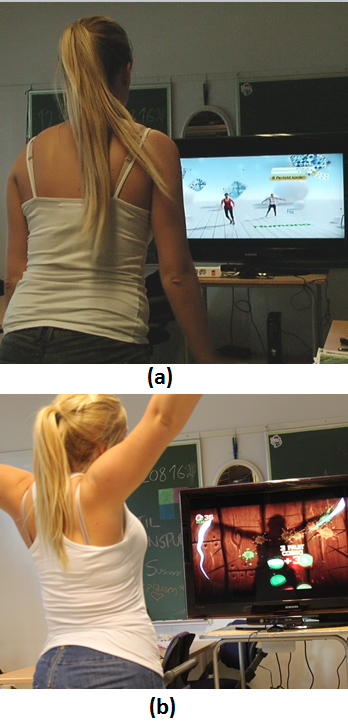
\includegraphics[scale=0.8]{delayx2.jpg}
\caption[Kinect sensor delay]{Figure (a) shows that there is a clear delay between the players movements and the avatar on the screen, while in figure (b) this delay is not present.}
\label{fig:remakeDelay}
\end{figure} 

\section{Quality of the Gathered Information}
\label{sec:qualityofresearch}

In Section \ref{sec:qualityresearch} the importance of evaluating quality of the research is discussed. This can be done by looking into the three criteria; \emph{reliability}, \emph{validity} and \emph{generalizability}.    

\subsection{Reliability}
Writing this report, we have distinguished between our own findings, and findings from theory and previous studies conducted by others. Our findings are presented in chapters separate from theory and literature, see Chapter \ref{chap:findW1} and \ref{chap:findW2}. In these chapters, neither our own opinions nor theory are included. These chapters only present feedback and opinions from the informants, as well as our observations. Citation is used were appropriate to strengthen our findings.  Findings from the two workshops are related to relevant theory in Chapter \ref{chap:concept}, where the exergame concept is presented, and earlier in this discussion chapter. This separation of information will strengthen the reliability of the information gathered.

The sample of informants chosen for our qualitative research might have affected the quality of our study. The informants are all members of "Seniornett", and are therefore very committed to learning about technology. All of them already use a wide range of technology devices. We evaluate them to be more experienced with technology than most people in the same age group. Most of the informants have a high education, and they are relatively active in their everyday life. Five out of seven informants stated that they are active in the means of exercise, while the two others mentioned that they are active due to everyday tasks. Based on this, we evaluate them as fit older people. The informants average age in workshop 1 was 70.6 years (with a standard deviation of 7,9 years), and 74,5 years (with a standard deviation of 7,5 years) in workshop 2. The informants are representative for our qualitative research based on their age span; however, they do not meet all the characteristics that are common for the older group. The exergame should also suit frail elderly people with different disabilities. This group of people might have experienced reduction in functionality, which makes it difficult to perform regular exercise and everyday tasks. 

Our relationship with the informants is an important aspects when discussing reliability. With the exception of one informant, we had never met the informants before. In addition, none of the informants knew each other. The fact that we were unknown for the informants could have resulted in the informants not wanting to say what they actually meant and felt. In addition, they might have experienced it as intimidating to talk to us. However, when first meeting the informants, we welcomed them and talked about familiar everyday topics, just making conversation. We felt this helped establish sort of a comfort. Our observation during the workshop, showed no sort of discomfort. They talked, laughed and joked a lot, both with us and each other, and we felt that the atmosphere was good. 

Our role in this workshop might have affected the reliability of our findings. What is preferred is for our participation to be neutral, but that was not the case. We participated in the workshop by informing about the technology, showing how the different games would work, we guided the informants when needed, and we partly participated in the discussion. This might have influenced the feedback from the informants. In addition, as we already have discussed, the fact that we presented our own concept, might have constrained the feedback. 


\subsection{Validity}

In the discussion we have related findings from the qualitative research with theory and previous studies within the same subject. What we see is that our results support what is found in related theory and findings. We did not experience much deviation in our findings from findings in previous studies. In addition, the outcome of our study forms a thorough basis for answering the research questions. We will therefore state that our findings are valid and of relevance to the purpose of the study. 

We had some difficulties placing our study within a specific research method, because what we have been studying is something completely new. By reading Chapter \ref{chap:metode} it should be clear for the reader which strategies and methods we have chosen to use, and why. We feel that this strengthen the validity of the information gathered. 
    
\subsection{Generalizability}    
The system requirements proposed in this thesis are based on thorough research with the use of a wide range of sources and data gathering methods. This makes the result so general, that it could be used as guidelines for others who want to develop similar games for the same user group. Many of the requirements can be used for the development of different types of user-interfaces for elderly people as well. Conceptual generalizability, which is the goal with the \ac{sdi} analysing method \cite{tjora}, can therefore be seen as relevant for this study. 

\subsection{Other Quality Aspects}
During this thesis we have given a detailed presentation of the theory used, the work we have done and the choices we have made. We have summarised theory to provide an accessible overview of the information for the reader, we have written in a familiar and easy-to-read language, and we have along the way discussed and justified all the theory we have used and choices we have made. As our report is written in a way that makes it easy for the reader to get insight into our work, it ensures transparency.

In our qualitative interviews we have used focus groups as setting. In Section \ref{sec:qualitativeInterviews} it is discussed that a preferred size for a focus group is 6-12 informants, but that mini-focus group interviews with 3-4 informants are accepted if the informants are experts on the discussed subject. Totally, we had seven informants for workshop 1, but these were divided into two days, with three and four informants each day. Theoretically, this means that we conducted mini-focus group interviews. The problem with this is that the informants are far from being experts on the subject, as they in fact never before had seen the technology we presented for them. However, what was a bit different with this first workshop was that we, in beforehand of the focus group interview, had introduced the informants for the Xbox Kinect technology. We asked about their perceived gaming experience in the interview, and felt that we received good, detailed and descriptive answers. 

One of the informants in the second workshop did not participate in workshop 1. This means that she attended workshop 2 with no previous experience with the Xbox Kinect technology, except from what we presented during our first meeting with "Seniornett". This made it difficult for her to relate to and understand what we presented during workshop 2, and she was therefore not able to provide us with much feedback. This is negative for the quality of the information gathered in workshop 2, as the number of involved informants already was less than what is preferred. 

In \ref{sec:otherQualityAspects} we present \emph{elite bias}, which is a pitfall that might have affected our results. Including only one group of people in qualitative research can give incomplete and under-representative data, and as a result, it could be hard to understand the broader situation. Because of the overall time limit for this master thesis, and other practical reasons, we only included this one group of people, even though they have the same interests for learning technology. Our findings would probably have been different if we had gathered a group of "random" people, because they would have more diversity in backgrounds and interests.

Another pitfall, presented in \ref{sec:otherQualityAspects}, that we might have experienced is the \emph{Hawthorn effect}. This is about the risk of people behaving differently because they know they are being observed. This may have been an issue in our qualitative research, since the Hawthorn effect may have an even bigger impact with the use of video recording. However, we tried to make a comfortable setting, and to "hide" the video recording equipment as much as possible. The informants seemed calm and unaffected by the video recording, and we therefore conclude that the Hawthorn effect did not affect the quality of our work. 

User involvement is about involving users from the start to the end of the system development process. We only included the informants two times in the development process, to discover their needs and opinions, and to evaluate our design. Basically, in line with user-centered design, the informants should have been more involved. However, this was not done due to time constraints in this master thesis, and because the informants were inexperience with the technology. 

Workshop 1 was held over two days, but it was not executed exactly equally the two days. One day the informants got a little more instruction and guidance than the next day, some informants got to play longer than others, and not all the same questions were asked during the discussion. All this can have affected the findings from this workshop.  

Since we performed focus group interviews, the informants were influenced by each other's statements and opinions. They discussed an unfamiliar subject, and it seemed easy to just "mean the same" as the informant stating something. As we had two groups of informants, the informants within each group formed similar opinions, that not necessary was the same in the two groups.
   
The choice of games for workshop 1 was not a coincidence. Each game was chosen for a reason (see Section \ref{sec:chosengames}) and we wanted to trig different reactions. This could have affected the outcome of our research. Choosing different games might have changed the findings from our research. 

In this chapter, the findings and the results are discussed. The discussion justifies the choice of concept, and it recommends future work to be done. In addition, we provide a thorough discussion on the quality of our research. This should help the reader of this report understand how he or she can rely on our findings and results.


